%\chapter{開発プロセス}
\section{第1サイクル(5月1日〜7月3日)}

\begin{description}
\item[第1回フィールドワーク]\mbox{}
\end{description}
 我々は木古内町の観光産業と開発するアプリの方向性を考えるにあたり、木古内町観光の解決すべき問題点の発見を目的として木古内町でフィールドワークを行った。このフィールドワークでは、多角的に木古内町を観察するために函館市-木古内町間の交通手段をメンバー間で電車・自転車・車の3つに分担し、それぞれが観光者の視点に立って行った。木古内町でのフィールドワークを行って気づいたことは主に2点あり、まず1点目は、木古内町の観光情報が分散して存在していることである。そのため、木古内町に着いた際、どこで何ができるのか分かりにくかった。これは、前述の木古内町観光協会WebサイトやSNS、パンフレットなど多くのメディアで情報が発信されていることで観光情報が分散していて観光者に伝わっていないことや、情報提供するコンテンツが木古内の魅力的な部分を十分に伝えていないことが原因だと考えられる。気づいたことの2点目は、観光を終えた人々には観光の体験や思い出を友人などの親しい人に伝えたいというモチベーションがあるという点である。観光の体験や思い出を伝えるという行為には、その相手に観光地の良さ伝え、新たな観光客を呼び込む手がかりとなる要素を含んでおり、それをより魅力的に伝えるには写真を使うのが効果的である。しかしながら、多くの観光者はその写真はあまり整理を行っておらずそれを効果的に伝えられていない。以上の気づきを元に第1サイクルの開発を開始した。
\bunseki{細川椋太}

第1サイクルはプロジェクト発足から中間発表会用のポスターレビューまでとした。本サイクルでは第1回フィールドワークの経験から、木古内町の観光情報が分散していること、観光中に撮影した写真が整理されていないことを問題として定義した。最初の設計段階であがった案は以下の5つであり具体的な画面イメージを作成できたのはマップ画面、Webページを表示する画面、お散歩コースを表示する画面の3つである。これらの案に対するレビューを6月12日に外部講師の方から受けた結果、現在の提案に木古内らしさを加える必要があるとの指摘を受けた。
\begin{description}
\item[初期段階でのアプリ機能案]\mbox{}
\begin{itemize}
 \item マップ上に表示されたピンをタップすると吹き出しとして詳細情報をクイック表示する機能
 \item 吹き出しをタップするとお店のWebページへ画面遷移する機能
 \item 木古内町民しか知らないニュースや、木古内町の天気をマップ画面に表示する
 \item ユーザ同士で木古内町の写真を共有できる機能
 \item 木古内町観光協会が公開している木古内お散歩コースをマップの中に盛り込む
\end{itemize}
\end{description}

\begin{description}
\item[作成した画面イメージ(図5.1)]\mbox{}
\begin{itemize}
 \item 図5.1(a)は、マップ上にピンを配置し、そのピンをタップすると詳細情報が記載された吹き出しを表示する。また、スポットを検索できたり木古内町の天気を表示したり表示するピンのカテゴリを切り替えることができるなどの機能を備えた画面イメージである。
 \item 図5.1(b)は、図5.1(a)に表示してある吹き出しをタップすると画面遷移して表示される画面である。ここには、観光スポットの詳細情報としてお店のメニューや開店閉店時間、商品の写真などが記載されている。
 \item 図5.1(c)は、木古内町観光協会が公開しているお散歩コースを表示している画面イメージである。画面下のタブをタップするたびに、コース内容を切り替えることができ、お散歩コースの途中にある観光スポットを赤点で表示している。
\end{itemize}
\end{description}

\begin{figure}[htbp]
  \begin{center}
    \begin{tabular}{c}

      % 1
      \begin{minipage}{0.33\hsize}
        \begin{center}
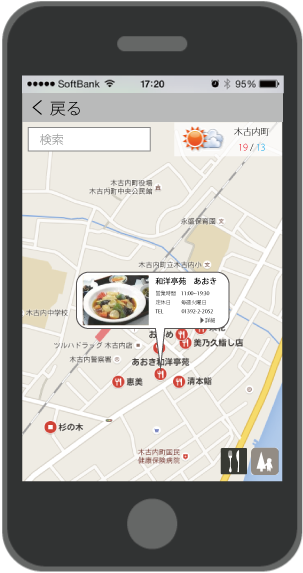
\includegraphics[width=4cm, bb=0 0 303 573]{5.2_map1.png}
          \hspace{1cm} (a)観光スポットの紹介
        \end{center}
      \end{minipage}

      % 2
      \begin{minipage}{0.33\hsize}
        \begin{center}
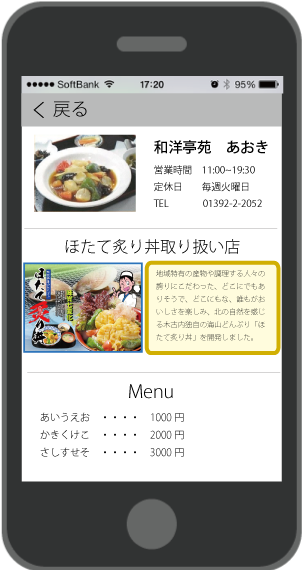
\includegraphics[width=4cm, bb=0 0 304 570]{5.2_map2.png}
          \hspace{1cm} (b)観光スポットの詳細情報
        \end{center}
      \end{minipage}

      % 3
      \begin{minipage}{0.33\hsize}
        \begin{center}
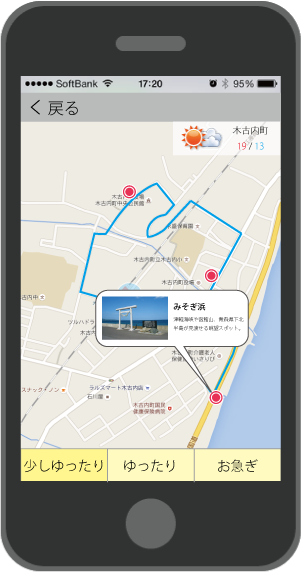
\includegraphics[width=4cm, bb=0 0 302 572]{5.2_sanpo.png}
          \hspace{1cm} (c)お散歩コース
        \end{center}
      \end{minipage}

    \end{tabular}
    \caption{初期段階での画面イメージ}
    \label{fig:lena}
  \end{center}
\end{figure}

その後は上記5つの案に対して議論を行い、木古内町民しか知らないニュースは継続運用が困難であるという理由から実装を保留した。また、木古内町観光協会が公開している木古内お散歩コースをマップの中に盛り込む機能については、公開されていたコース内容が車での移動を前提にしており、自分たちでコースを作らなければいけないという理由から実装は保留となった。この段階で実装した機能は下記の3つである。しかし、中間発表会用のポスターレビューの際にユーザストーリに問題があるとの指摘を受けた。具体的には、観光客は観光スポットやランドマークの写真を見てからその場所へ行くのが通常の流れである。しかし、当時作成していたアプリは場所を伝えてから写真や詳細情報を見せる流れになってしまっていた。この状態だと木古内町の魅力はもちろんのこと、何があるかすら伝わらないとの内容であった。この指摘を受けて先に伝える情報は場所ではなく内容にすべきという結論に達した。そして中間発表会までに改善することをメンバー間で合意し、第2サイクルへ移行した。
\begin{description}
\item[第1サイクルで実装した機能]\mbox{}
\begin{itemize}
 \item マップ上に表示されたピンをタップすると吹き出しとして詳細情報をクイック表示する機能
 \item 現在地から目的地までのルート案内
 \item 木古内町の天気を表示する
\end{itemize}
\end{description}

\begin{description}
\item[画面の詳細説明(図5.2)]\mbox{}
\begin{itemize}
 \item 図5.2(a)はユーザが一番最初に見る画面である。画面にはマップが大きく表示されており、画面下には食べる、見る、買うの3つのカテゴリがボタンとして表示してある。各カテゴリをタップするとマップ上に表示されるピンが切り替わる仕組みだ。また、表示されているピンをタップするとスポットの名前と連絡先が記載された吹き出しを表示する。
 \item 図5.2(b)は、現在地からスポットまでのルートを表示している画面である。図5.2(a)中にある吹き出し右側に表示している青いアイコンをタップすることでルートが赤線で表示される。
 \item 図5.2(c)は、木古内町の天気を表示している画面である。現在の最高気温及び最低気温、3時間ごとの天気、1週間の天気予報を表示している。
\end{itemize}
\end{description}

\begin{figure}[htbp]
  \begin{center}
    \begin{tabular}{c}

      % 1
      \begin{minipage}{0.33\hsize}
        \begin{center}
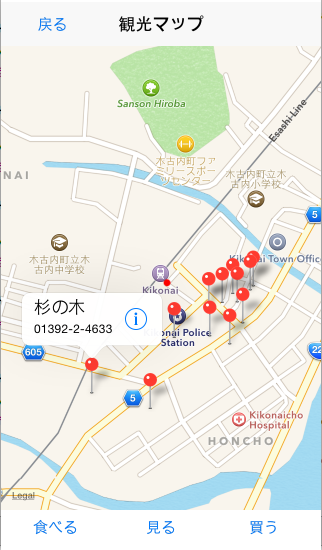
\includegraphics[width=4cm, bb=0 0 322 550]{5.3_map1.png}
          \hspace{1cm} (a)詳細情報のクイック表示
        \end{center}
      \end{minipage}

      % 2
      \begin{minipage}{0.33\hsize}
        \begin{center}
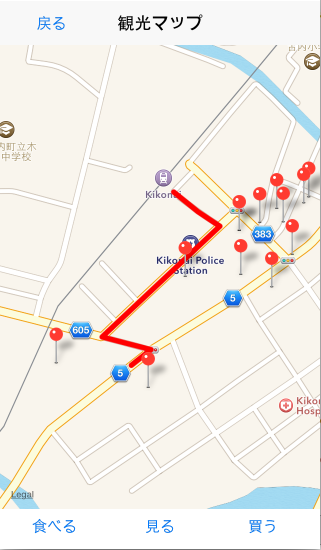
\includegraphics[width=4cm, bb=0 0 321 550]{5.3_map2.png}
          \hspace{1cm} (b)ルート案内
        \end{center}
      \end{minipage}

      % 3
      \begin{minipage}{0.33\hsize}
        \begin{center}
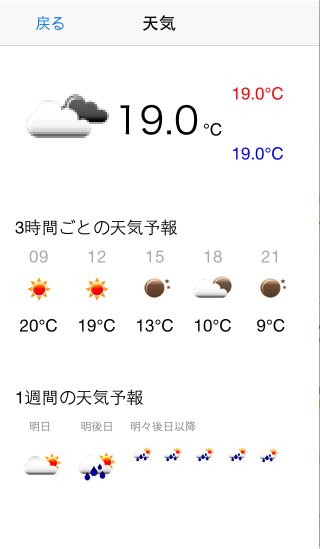
\includegraphics[width=4cm, bb=0 0 320 549]{5.3_weather.png}
          \hspace{1cm} (c)木古内町の天気を表示
        \end{center}
      \end{minipage}

    \end{tabular}
    \caption{第1サイクルでの完成画面 }
    
    \label{fig:lena}
  \end{center}
\end{figure}
\bunseki{岩見建汰}